\documentclass[11pt,a4paper]{article}
\usepackage[margin=23mm,headheight=15pt]{geometry}
\usepackage[T1]{fontenc}
\usepackage{lmodern}
\usepackage{tgpagella}
\usepackage{amsmath,amssymb,amsthm,mathtools,bm}
\usepackage{microtype,booktabs,longtable,tabularx,array,enumitem}
\usepackage{tikz}
\usetikzlibrary{arrows.meta,positioning,calc,decorations.pathmorphing,patterns}
\usepackage{fancyhdr,xcolor,hyperref}
\definecolor{deepblue}{RGB}{25,50,99}
\definecolor{purple}{RGB}{104,69,170}
\definecolor{softblue}{RGB}{225,237,251}
\hypersetup{colorlinks=true,urlcolor=deepblue,linkcolor=deepblue}
\pagestyle{fancy}\fancyhf{}\fancyhead[L]{\small Rubidium-87: Atomic Orbitals and Quantum Condensation}\fancyhead[R]{\small Quantum Physics Companion}\fancyfoot[C]{\thepage}
\setlength{\parskip}{5pt}\setlength{\parindent}{0pt}
\setcounter{secnumdepth}{3}
\newtheorem{example}{Worked Example}
\newtheorem{remark}{Remark}
\newcommand{\Rb}{^{87}\mathrm{Rb}}
\newcommand{\kb}{k_{\mathrm B}}
\newcommand{\ph}{\varphi}
\newcommand{\dd}{\mathrm d}
\newcommand{\cm}{\mathrm{CM}}
\begin{document}
\begin{center}
{\Large\bfseries\color{deepblue} From Rubidium Atomic Orbitals\\ to a Macroscopic Quantum Wave}\par\medskip
{\large An Extended Companion Chapter with Derivations, Diagrams and Worked Examples}\\[4pt]
{\small 17 November 2026 \quad $\cdot$ \quad Atomic structure, Bose statistics, coherence, interferometry and electronic bands}
\end{center}
\vspace{3mm}
\begin{abstract}
This chapter explains how thousands of neutral $\Rb$ atoms can occupy one coherent motional quantum state without merging their nuclei or electronic orbitals. Starting from the electron configuration $[\mathrm{Kr}]5s^1$, we distinguish internal electronic and external center-of-mass wavefunctions, derive atomic transition selection rules, build the Bose many-body state in first and second quantization, introduce the Penrose--Onsager criterion and Gross--Pitaevskii dynamics, calculate laboratory energy and length scales, and contrast ultracold quantum gases with electronic band formation in crystals. The November 2026 Tiangong experiment provides a contemporary experimental context; its picokelvin number is an equivalent expansion-energy temperature, not a thermometer reading for the entire apparatus.
\end{abstract}
\tableofcontents
\newpage
\section{The physical question and three levels of description}
A neutral $\Rb$ atom contains 37 protons, 50 neutrons and 37 electrons. Yet a dilute cloud of approximately $2\times 10^4$ such atoms can exhibit macroscopic occupation of a single center-of-mass quantum mode. The word \emph{orbital} is used in two distinct settings. An electronic orbital is a wavefunction of an electron relative to its nucleus and other electrons; a motional orbital is a wavefunction for the \emph{whole atom's} center of mass in an external potential. Their characteristic length and energy scales differ drastically.

For a well-defined internal state and weak internal--external coupling, a single-atom wavefunction can be approximated by
\begin{equation}
\Psi_{\mathrm{atom}}(\mathbf R,\boldsymbol\xi) \simeq \ph_{\cm}(\mathbf R)\chi_{\mathrm{int}}(\boldsymbol\xi),
\label{eq:factor}
\end{equation}
where $\mathbf R$ is the atomic center of mass and $\boldsymbol\xi$ denotes all internal relative coordinates and spins. This factorization is approximate: polarization forces, state-dependent trapping, recoil and collisions can couple the two factors.

\begin{center}
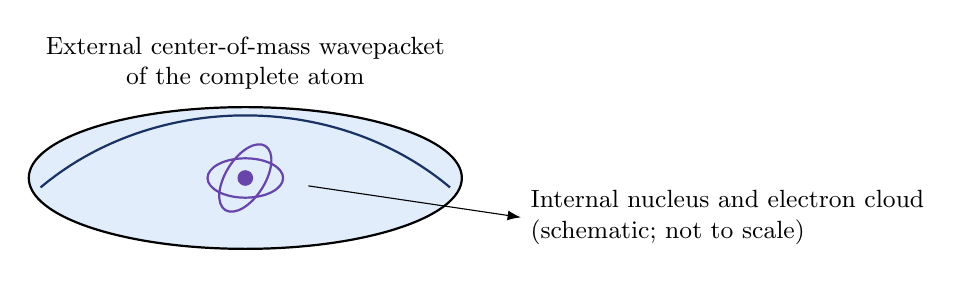
\begin{tikzpicture}[>=Latex,font=\small]
\draw[thick,fill=softblue] (0,0) ellipse (2.75 and 0.9);
\draw[deepblue,thick] (-2.6,-.12) .. controls (-1.15,1.1) and (1.15,1.1) .. (2.6,-.12);
\node[fill=purple,circle,inner sep=2pt] at (0,0) {};
\draw[purple,thick] (0,0) ellipse (.48 and .25);
\draw[purple,thick,rotate around={58:(0,0)}] (0,0) ellipse (.48 and .25);
\node[align=center,above] at (0,1.0) {External center-of-mass wavepacket\\of the complete atom};
\draw[->] (0.8,-.1) -- (3.5,-.5);
\node[align=left,right] at (3.5,-.5) {Internal nucleus and electron cloud\\(schematic; not to scale)};
\end{tikzpicture}
\end{center}

\section{Rubidium-87 electronic structure}
\subsection{Electron configuration and orbitals}
In its electronic ground state, neutral rubidium has
\begin{equation}
1s^2\,2s^2\,2p^6\,3s^2\,3p^6\,3d^{10}\,4s^2\,4p^6\,5s^1=[\mathrm{Kr}]5s^1.
\end{equation}
The shell populations are $2,8,18,8,1$. The last electron is in a $5s$ state. The $s,p,d,f$ labels indicate orbital angular momentum $\ell=0,1,2,3$. In a central potential,
\begin{equation}
\psi_{n\ell m}(\mathbf r)=R_{n\ell}(r)Y_{\ell}^{m}(\theta,\phi),\quad \int |\psi_{n\ell m}|^2\dd^3r=1.
\end{equation}
The $s$-state electronic probability density is spherically symmetric, but the radial wavefunction has structure. A hydrogenic $5s$ radial state has $n-\ell-1=4$ radial nodes. Rubidium is not a hydrogen atom: core screening, penetration, exchange and spin--orbit interactions make a quantitatively accurate $R_{5s}$ a many-electron atomic-structure problem. It is therefore incorrect to draw the $5s$ state as a simple electron circling a fixed spherical path.

\subsection{Spin, fine structure and hyperfine structure}
The valence electron has $s=1/2$ and $\mathbf J=\mathbf L+\mathbf S$. The relevant terms are $5^2S_{1/2}$, $5^2P_{1/2}$, and $5^2P_{3/2}$. The $\Rb$ nucleus has spin $I=3/2$. Hyperfine total angular momentum is $\mathbf F=\mathbf I+\mathbf J$. Thus the $5S_{1/2}$ manifold has $F=1,2$; the $5P_{1/2}$ manifold has $F'=1,2$; and the $5P_{3/2}$ manifold has $F'=0,1,2,3$.

The leading hyperfine magnetic-dipole interaction is $H_{\rm hfs}=A\mathbf I\cdot\mathbf J$, whose level energy is
\begin{equation}
E_F=\frac{A}{2}[F(F+1)-I(I+1)-J(J+1)],
\end{equation}
with additional quadrupole contributions for certain $J\geq1$ states. The $5S_{1/2}$ ground-state $F=1\leftrightarrow F=2$ splitting is approximately $6.834682611$ GHz.

\begin{center}
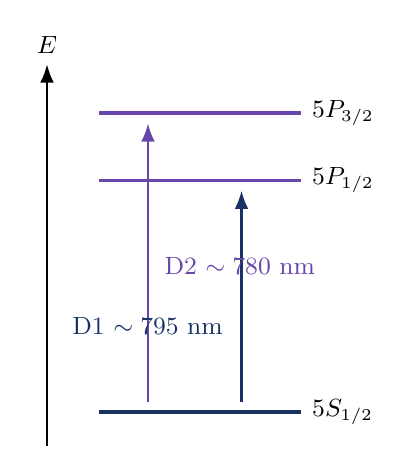
\begin{tikzpicture}[font=\small,>=Latex,scale=.95]
\draw[->,thick] (0,0)--(0,5.1) node[above]{$E$};
\draw[very thick,purple] (.7,4.45)--(3.4,4.45) node[right,black]{$5P_{3/2}$};
\draw[very thick,purple] (.7,3.55)--(3.4,3.55) node[right,black]{$5P_{1/2}$};
\draw[very thick,deepblue] (.7,.45)--(3.4,.45) node[right,black]{$5S_{1/2}$};
\draw[->,thick,purple] (1.35,.59)--(1.35,4.31);
\draw[->,thick,deepblue] (2.6,.59)--(2.6,3.41);
\node[purple,anchor=west] at (1.44,2.4) {D2 $\sim780$ nm};
\node[deepblue,anchor=east] at (2.48,1.6) {D1 $\sim795$ nm};
\end{tikzpicture}
\end{center}

\subsection{Electric-dipole selection rules}
The light--matter interaction in the electric dipole approximation is $H'(t)=-\mathbf d\cdot\mathbf E(t)$. A transition amplitude is proportional to $\langle f|\mathbf d\cdot\boldsymbol\epsilon|i\rangle$. The orbital-parity rule requires opposite parity, with $\Delta\ell=\pm1$. For fine-structure angular momentum, the usual electric-dipole rule is $\Delta J=0,\pm1$ except $J=0\not\leftrightarrow J'=0$. For resolved hyperfine transitions, $\Delta F=0,\pm1$ except $F=0\not\leftrightarrow F'=0$, with polarization-dependent $\Delta m_F=0,\pm1$.

These rules explain why $5S\to5P$ is dipole allowed, while $5S\to5S$ is not an ordinary one-photon electric-dipole transition. Real cooling transitions also require attention to optical pumping and repumping among hyperfine levels.

\begin{example}[D2 photon energy and atomic momentum recoil]
For $\lambda=780\,$nm,
\[E_\gamma=hc/\lambda\simeq2.55\times10^{-19}\,\mathrm J\simeq1.59\,\mathrm{eV}.\]
The photon momentum is $p_\gamma=h/\lambda\simeq8.49\times10^{-28}\,\mathrm{kg\,m/s}$. For $M\simeq1.443\times10^{-25}\,$kg, the recoil velocity is $v_r=p_\gamma/M\simeq5.89\,$mm/s. The recoil energy is $E_r=p_\gamma^2/(2M)$, corresponding to $E_r/\kb\simeq181\,$nK. A large optical excitation energy can therefore coexist with a much smaller motional recoil energy.
\end{example}

\begin{example}[Ground-state hyperfine energy]
The $6.83468$ GHz separation corresponds to $\Delta E=h\nu\simeq4.53\times10^{-24}\,$J or an equivalent $\Delta E/\kb\simeq0.328\,$K. This is again vastly larger than a nanokelvin-scale center-of-mass kinetic energy. Microwave driving can change a hyperfine state without necessarily changing the electronic principal shell.
\end{example}

\section{Internal vs external degrees of freedom}
Write the exact many-particle kinetic energy using the atomic center of mass $\mathbf R$ and internal relative coordinates $\boldsymbol\xi$. For an isolated atom, translational invariance allows separation $H_{\rm atom}=\mathbf P^2/(2M)+H_{\rm int}$. In a trap, one instead has
\begin{equation}
H\simeq H_{\rm int}+\left[-\frac{\hbar^2}{2M}\nabla_{\mathbf R}^2+V_{\rm trap}(\mathbf R)\right]+H_{\rm coupl}.
\end{equation}
The center-of-mass state $\ph(\mathbf R)$ can spread over tens of micrometres without the electron cloud swelling to the same size. At every possible $\mathbf R$, the atom retains essentially its local internal state $\chi_{\rm int}$. An $\Rb$ condensate is therefore not a chemically giant atom.

For one harmonic trapping axis, $V(X)=M\omega^2X^2/2$ and
\begin{equation}
E_n=\hbar\omega(n+1/2),\qquad a_{\rm ho}=\sqrt{\frac{\hbar}{M\omega}},\qquad
\ph_0(X)=\frac{e^{-X^2/(2a_{\rm ho}^2)}}{\pi^{1/4}\sqrt{a_{\rm ho}}}.
\end{equation}
These $n=0,1,2,\ldots$ labels describe trap states of \emph{the entire atom}. They are not the electronic $n=1,2,3,\ldots$ shell labels.

\begin{example}[Size of a motional orbital]
For $\omega=2\pi\times10\,$s$^{-1}$ and $M=1.443\times10^{-25}\,$kg, $a_{\rm ho}=\sqrt{\hbar/(M\omega)}\simeq3.41\,\mu$m. That length is thousands of times larger than the typical size of the electronic structure, yet it represents the spatial uncertainty of the atom's center of mass, not an electronic shell radius.
\end{example}

\section{Bosonic exchange symmetry and occupation numbers}
Rubidium-87 has an integer total spin for the complete atom and behaves as a composite boson in the cold-atom regime. For identical bosons, the many-body wavefunction is symmetric under particle exchange. For two atoms in distinct orthonormal orbitals,
\begin{equation}
\Phi_{ab}(1,2)=\frac{\ph_a(1)\ph_b(2)+\ph_b(1)\ph_a(2)}{\sqrt2}.
\end{equation}
For two bosons in the \emph{same} orbital, the normalized wavefunction is $\ph_0(1)\ph_0(2)$, with no exclusion principle violation. For $N$ noninteracting atoms occupying one orbital,
\begin{equation}
\Phi_N(\mathbf R_1,\ldots,\mathbf R_N)=\prod_{j=1}^{N}\ph_0(\mathbf R_j),\qquad \int |\ph_0|^2\dd^3R=1.
\end{equation}
It remains an $N$-coordinate wavefunction. In second quantization, the corresponding occupation-number state is
\begin{equation}
|N_0\rangle=\frac{(\hat a_0^\dagger)^{N_0}}{\sqrt{N_0!}}|0\rangle,\qquad [\hat a_j,\hat a_k^\dagger]=\delta_{jk}.
\end{equation}
The operator $\hat a_0^\dagger$ creates a \emph{whole atom} in a motional state $\ph_0$; it never means creating a new electron in a common $5s$ shell.

\subsection{Bose statistics and critical temperature}
For ideal bosons in a grand-canonical description,
\begin{equation}
\bar n_j=\frac{1}{\exp[(\epsilon_j-\mu)/(\kb T)]-1}.
\end{equation}
The chemical potential of the ideal gas approaches the lowest one-particle energy from below as the condensed population develops. In a uniform three-dimensional ideal gas, the critical phase-space density is
\begin{equation}
n\lambda_{\rm th}^3=\zeta(3/2)\simeq2.612,\qquad
\lambda_{\rm th}=\frac{h}{\sqrt{2\pi M\kb T}}.
\end{equation}
For an ideal gas in a three-dimensional harmonic trap, with geometric mean trap frequency $\bar\omega$, a large-$N$ approximation gives $\kb T_c\simeq\hbar\bar\omega[N/\zeta(3)]^{1/3}$. Interactions and finite size shift the actual transition.

\begin{example}[Ideal harmonically trapped transition]
For $N=20{,}000$ and $\bar\omega=2\pi\times100\,$s$^{-1}$, the ideal formula gives $T_c\simeq1.23\times10^{-7}\,$K $=123\,$nK. This is an illustrative trap, not a measurement of Tiangong's initial trapping frequencies or critical temperature.
\end{example}

\section{Condensation via the one-body density matrix}
A macroscopic occupation criterion is more robust than simply drawing overlapping Gaussians. The field operator is
\begin{equation}
\hat\psi(\mathbf R)=\sum_j\ph_j(\mathbf R)\hat a_j.
\end{equation}
The one-body density matrix is
\begin{equation}
\rho_1(\mathbf R,\mathbf R')=\langle\hat\psi^\dagger(\mathbf R')\hat\psi(\mathbf R)\rangle.
\end{equation}
Its spectral decomposition is
\begin{equation}
\rho_1(\mathbf R,\mathbf R')=\sum_j N_j\ph_j(\mathbf R)\ph_j^*(\mathbf R'),\qquad\sum_jN_j=N.
\end{equation}
The Penrose--Onsager criterion states that a one-body eigenvalue $N_0=O(N)$ signals Bose--Einstein condensation. $\ph_0$ is called the condensate natural orbital. In interacting systems the exact many-body state need not be a product of $N$ identical single-atom orbitals. Quantum depletion and correlations can coexist with a macroscopically occupied natural orbital.

A phase-based description writes $\Psi(\mathbf R,t)\simeq\sqrt{N_0}\ph_0(\mathbf R,t)=\sqrt{n_0}\,e^{i\theta}$. A number eigenstate need not have a nonzero anomalous expectation $\langle\hat\psi\rangle$; an order parameter is nonetheless useful in symmetry-broken or relative-phase descriptions. Observable interference depends on phase \emph{differences}, not on a physically accessible absolute global phase.

\begin{example}[Condensate fraction and natural-orbital occupations]
Suppose $N=20{,}000$ and the largest eigenvalue of $\rho_1$ is $N_0=18{,}000$. Then $f_0=N_0/N=0.90$; the remaining 2,000 atoms populate other natural orbitals. This is an invented numerical demonstration, not a claimed measured condensate fraction aboard Tiangong.
\end{example}

\section{Contact interactions and Gross--Pitaevskii dynamics}
For a weakly interacting dilute single-component Bose gas, low-energy two-body scattering is characterized by an $s$-wave scattering length $a_s$. A contact model replaces the microscopic potential by $g\delta(\mathbf R-\mathbf R')$, with
\begin{equation}
g=\frac{4\pi\hbar^2a_s}{M}.
\end{equation}
A commonly prepared $\Rb$ state has positive $a_s\simeq5.3\,$nm, though this is state- and field-dependent. In second quantization,
\begin{equation}
\hat H=\int\dd^3R\,\hat\psi^\dagger\left(-\frac{\hbar^2\nabla^2}{2M}+V\right)\hat\psi+
\frac g2\int\dd^3R\,\hat\psi^\dagger\hat\psi^\dagger\hat\psi\hat\psi.
\end{equation}
A coherent mean-field approximation yields the Gross--Pitaevskii equation
\begin{equation}
\boxed{\ i\hbar\partial_t\Psi=\left[-\frac{\hbar^2}{2M}\nabla^2+V(\mathbf R,t)+g|\Psi|^2\right]\Psi\ },\qquad \int|\Psi|^2\dd^3R=N_0.
\label{eq:gpe}
\end{equation}
For a stationary state $\Psi(\mathbf R,t)=\psi_0(\mathbf R)e^{-i\mu t/\hbar}$,
\begin{equation}
\mu\psi_0=\left[-\frac{\hbar^2}{2M}\nabla^2+V+g|\psi_0|^2\right]\psi_0.
\end{equation}
The chemical potential $\mu$ is not generally the bare lowest harmonic oscillator energy when interactions matter. In the Thomas--Fermi regime, dropping the kinetic-energy term in the stationary density equation gives
\begin{equation}
n(\mathbf R)\simeq\max\left\{\frac{\mu-V(\mathbf R)}{g},0\right\}.
\end{equation}

\subsection{Density, phase, current and quantized circulation}
Set $\Psi=\sqrt n\,e^{i\theta}$. The GPE implies the continuity equation $\partial_t n+\nabla\cdot(n\mathbf v)=0$, where $\mathbf v=(\hbar/M)\nabla\theta$. For a closed loop without singularities, single-valuedness of $\Psi$ gives
\begin{equation}
\oint\mathbf v\cdot\dd\mathbf l=\frac{\hbar}{M}\oint\nabla\theta\cdot\dd\mathbf l=\frac{2\pi\hbar}{M}q=\frac hM q,\quad q\in\mathbb Z.
\end{equation}
This is why a BEC can display quantized vortices: the phase has experimentally meaningful spatial structure. It is not merely a uniform color assigned to all atoms.

\begin{example}[Quantized circulation in a rubidium condensate]
For one phase winding, $\kappa=h/M\simeq4.59\times10^{-9}\,\mathrm{m^2/s}$. The sign follows the orientation of the vortex; the magnitude is fixed by Planck's constant and the atomic mass.
\end{example}

\section{Expansion, equivalent temperature and microgravity}
\subsection{Time of flight and interpretation}
After releasing a gas from its trap, its density expands. For a noninteracting cloud with no initial position--velocity correlations, the variance obeys $\sigma_x^2(t)=\sigma_x^2(0)+\sigma_{v_x}^2t^2$. If an observed asymptotic one-dimensional expansion variance can be treated as a thermal kinetic variance, one defines
\begin{equation}
T_{\rm eq,x}=\frac{M\sigma_{v_x}^2}{\kb}.
\end{equation}
This definition is an \emph{equivalent expansion-energy temperature}; it need not be identical to a thermodynamic equilibrium temperature. A condensate may expand from both kinetic pressure and repulsive mean-field interactions. Thus measured profiles must be interpreted using the actual experimental dynamics, and the above simple variance model is only a pedagogical baseline.

\begin{example}[Velocity scale associated with a 9.7-pK equivalent temperature]
In one dimension, $\sigma_v=\sqrt{\kb T_{\rm eq}/M}$. For $T_{\rm eq}=9.7\times10^{-12}\,$K and $M=1.443\times10^{-25}\,$kg, $\sigma_v\simeq3.05\times10^{-5}\,$m/s $=30.5\,\mu$m/s. If this ballistic velocity spread persisted over seven seconds, its contribution to width would be roughly $214\,\mu$m. This is an illustrative conversion, not a reproduction of the experiment's multidimensional fitting procedure.
\end{example}

\begin{example}[Formal wavelength comparison]
The ideal-gas expression $\lambda_{\rm th}=h/\sqrt{2\pi M\kb T}$ gives $\lambda_{\rm th}\simeq0.593\,\mu$m at $100\,$nK and $\simeq59.3\,\mu$m at $10\,$pK. The latter is only a formal energy--wavelength conversion: the Tiangong equivalent expansion temperature does not establish a thermal equilibrium distribution at 10 pK.
\end{example}

\subsection{Why microgravity helps}
A freely falling orbital laboratory largely suppresses the relative acceleration of atoms against its apparatus. A seven-second free fall under Earth's surface gravity would have a displacement $gt^2/2\simeq240\,$m. Orbital microgravity permits extended free evolution within a compact science module, although residual gradients, spacecraft disturbances, fields and optical imperfections still matter.

The November 2026 Science report describes an ODT-based BEC of $2.0\times10^4$ atoms with equivalent temperature $9.7^{+3.2}_{-2.7}$ pK and $7.0\,$s expansion. This is a measurement of slow atomic expansion; the spacecraft itself and the complete experimental apparatus were not cooled to picokelvin temperatures.

\section{Coherence and interferometry}
Two coherently split wavepackets $\Psi_A=|\Psi_A|e^{i\theta_A}$ and $\Psi_B=|\Psi_B|e^{i\theta_B}$ produce intensity/density
\begin{equation}
|\Psi_A+\Psi_B|^2=|\Psi_A|^2+|\Psi_B|^2+2|\Psi_A||\Psi_B|\cos(\theta_A-\theta_B).
\end{equation}
The cross-term is the interference signal. It directly measures a relative phase when the modes overlap and detection resolves the fringes. In a common three-pulse light-pulse atom interferometer, a uniform acceleration contributes approximately $\Delta\phi=\mathbf k_{\rm eff}\cdot\mathbf a\,T^2$, subject to the geometry and pulse sequence.

\begin{example}[Interferometer interrogation-time scaling]
Holding $k_{\rm eff}$ and acceleration fixed, changing the pulse separation from $T=1\,$s to $T=7\,$s multiplies the ideal acceleration-dependent phase by $49$. Longer times are not automatically 49 times more precise: contrast, wavepacket overlap, technical noise and systematics determine the achieved sensitivity.
\end{example}

\section{Why an atomic BEC is not an electronic crystal}
Two very different overlaps must be separated. First, a dilute gas of neutral atoms has overlapping \emph{center-of-mass probability amplitudes}; the atoms can macroscopically occupy one motional natural orbital. Second, in a solid, neighboring atoms' \emph{electronic} wavefunctions can overlap strongly enough to generate hopping and hybridized band states. The latter is fundamentally an electronic-structure problem.

For a periodic crystalline potential $V(\mathbf r+\mathbf a)=V(\mathbf r)$, Bloch's theorem gives
\begin{equation}
\psi_{n\mathbf k}(\mathbf r)=e^{i\mathbf k\cdot\mathbf r}u_{n\mathbf k}(\mathbf r),\quad u_{n\mathbf k}(\mathbf r+\mathbf a)=u_{n\mathbf k}(\mathbf r).
\end{equation}
A nearest-neighbor tight-binding band on a one-dimensional lattice has $E(k)=\epsilon_0-2t\cos(ka)$. The hopping $t$ arises from matrix elements between orbitals centered at neighboring lattice sites. Rubidium metal is a real example of a solid with a partially filled electronic band derived in part from atomic valence states.

\begin{center}
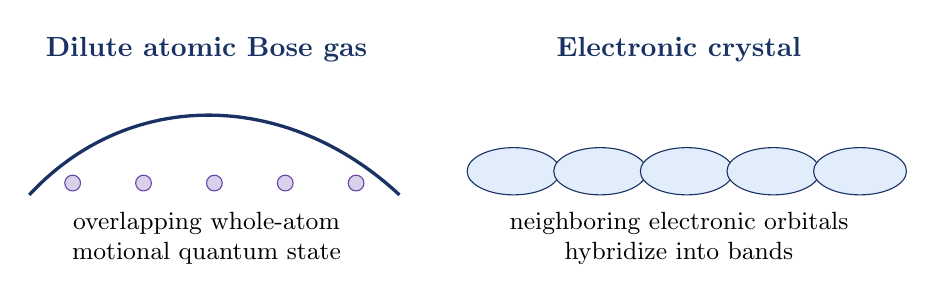
\begin{tikzpicture}[>=Latex,font=\small]
\node[deepblue,font=\bfseries] at (2,2.2) {Dilute atomic Bose gas};
\foreach \x in {0.3,1.2,2.1,3.0,3.9} {\draw[fill=purple!25,draw=purple] (\x,.5) circle (.10);}
\draw[very thick,deepblue] (-.25,.35) .. controls (1,1.7) and (3,1.7) .. (4.45,.35);
\node[align=center] at (2,-.2) {overlapping whole-atom\\motional quantum state};
\node[deepblue,font=\bfseries] at (8.0,2.2) {Electronic crystal};
\foreach \x in {5.9,7.0,8.1,9.2,10.3} {\draw[fill=purple!20,draw=purple] (\x,.65) circle (.2);\draw[deepblue,fill=softblue] (\x,.65) ellipse (.59 and .30);}
\node[align=center] at (8,-.2) {neighboring electronic orbitals\\hybridize into bands};
\end{tikzpicture}
\end{center}

An optical lattice offers a further distinction: it creates a periodic potential for the centers of mass of ultracold atoms, often leading to a Bose--Hubbard Hamiltonian
\begin{equation}
\hat H_{\rm BH}=-J\sum_{\langle i,j\rangle}(\hat b_i^\dagger\hat b_j+\mathrm{h.c.})+\frac U2\sum_i\hat n_i(\hat n_i-1)+\sum_i(V_i-\mu)\hat n_i.
\end{equation}
Here the Wannier orbitals describe trapped \emph{whole atoms} in optical potential wells, not their internal electronic $5s$ orbitals. Thus a gas in an optical lattice is an especially useful bridge between condensed matter and atomic BEC physics, but the microscopic degrees of freedom must not be confused.

\begin{example}[Tight-binding band width versus Bose occupation]
In the one-dimensional electronic tight-binding model $E(k)=\epsilon_0-2t\cos(ka)$, the band width is $4|t|$. This spreading of allowed \emph{electronic} energies is due to intersite orbital hopping. In a single-mode atomic BEC, by contrast, increasing $N_0$ from $10^3$ to $2\times10^4$ changes occupation of one \emph{motional} mode; it is not the generation of a 20,000-orbital electronic band.
\end{example}

\section{Synthesis and limitations}
We can now state the complete answer precisely. Each Rb atom retains its internal many-electron state $\chi_{\rm int}$. Laser transitions $5S\leftrightarrow5P$ change atomic electronic and hyperfine states and transfer momentum. Cooling and trapping control the center-of-mass states $\ph_j$. Identical bosonic atoms can macroscopically occupy one motional natural orbital $\ph_0$. Their condensate can be represented at mean-field level by $\Psi=\sqrt{n_0}e^{i\theta}$, evolving according to the GPE when its assumptions apply.

This description does not imply nuclear fusion, shared electronic shells, exact zero velocity or a literal many-body product state in a strongly correlated system. Absolute condensate phase is not independently observable; relative phases and correlation functions are. The $9.7$-pK space result is an exceptionally small equivalent expansion energy, and neither directly measures an absolute thermal equilibrium temperature nor forces all atomic motion to cease.

\subsection*{Key identities}
\begin{align*}
\psi_{n\ell m}(\mathbf r)&=R_{n\ell}(r)Y_\ell^m(\theta,\phi) &&\text{(electronic orbital)},\\
\Psi_{\rm atom}&\simeq\ph_{\rm CM}\chi_{\rm int}&&\text{(internal/external separation)},\\
|N_0\rangle&=(\hat a_0^\dagger)^{N_0}|0\rangle/\sqrt{N_0!}&&\text{(bosonic occupation)},\\
\rho_1(\mathbf R,\mathbf R')&=\langle\hat\psi^\dagger(\mathbf R')\hat\psi(\mathbf R)\rangle&&\text{(one-body density matrix)},\\
\Psi_{\rm BEC}&=\sqrt{n_0}e^{i\theta}&&\text{(order parameter)},\\
\mathbf v&=(\hbar/M)\nabla\theta&&\text{(superfluid velocity)}.
\end{align*}

\section*{Further problems}
\begin{enumerate}[leftmargin=*]
\item Compute the electronic $5s\to5p$ photon frequencies from the D1 and D2 wavelengths and compare their difference with the ground hyperfine splitting.
\item Starting from $\ph_0(X)$ for a harmonic trap, prove its normalization and find $\langle X^2\rangle$.
\item Derive the ideal-gas phase-space condition $n\lambda_{\rm th}^3=\zeta(3/2)$ by integrating the Bose distribution in momentum space.
\item Show that $\langle\hat\psi\rangle=0$ for a fixed-number condensate while $\rho_1$ still has a macroscopic eigenvalue.
\item Substitute $\Psi=\sqrt{n}e^{i\theta}$ into the GPE and derive the continuity equation and quantum-pressure term.
\item Compare $E(k)$ for a tight-binding electron with the lowest Wannier mode of a neutral atom in an optical lattice. Identify the different physical particles.
\end{enumerate}

\section*{References and measurement notes}
\begingroup\sloppy
\begin{enumerate}[leftmargin=*]
\item W. Xiong et al., ``Quantum gases below 10 picokelvin in space,'' \emph{Science}, online 5 November 2026, DOI: \href{https://doi.org/10.1126/science.aea5324}{10.1126/science.aea5324}; abstract indexed at \url{https://pubmed.ncbi.nlm.nih.gov/42986982/}.
\item D. A. Steck, \emph{Rubidium 87 D Line Data}, \url{https://steck.us/alkalidata/rubidium87numbers.pdf}. Numerical transition and hyperfine reference.
\item Chinese Academy of Sciences, ``China's Space Station Sets New Atomic Cooling Record,'' 6 November 2026, \url{https://english.cas.cn/newsroom/cas-in-media/202611/t20261106_1213502.shtml}.
\item F. Dalfovo, S. Giorgini, L. P. Pitaevskii and S. Stringari, ``Theory of Bose--Einstein condensation in trapped gases,'' \emph{Reviews of Modern Physics} 71 (1999), 463--512.
\item C. J. Pethick and H. Smith, \emph{Bose--Einstein Condensation in Dilute Gases}, Cambridge University Press.
\end{enumerate}
\endgroup

\clearpage
\section*{Supplementary Sections to Chapter I: deeper explanations (original chapter preserved)}
\addcontentsline{toc}{section}{Supplementary Sections to Chapter I}
\subsection*{I-A. Separation of atomic center-of-mass and internal coordinates}
For an atomic nucleus of mass $M_N$ and $Z$ electrons, the full nonrelativistic Hamiltonian (before including fine-structure corrections) is
\begin{equation}
H=\frac{\mathbf P_N^2}{2M_N}+\sum_{i=1}^{Z}\frac{\mathbf p_i^2}{2m_e}
-\sum_i\frac{Ze^2}{4\pi\epsilon_0|\mathbf r_i-\mathbf r_N|}
+\sum_{i<j}\frac{e^2}{4\pi\epsilon_0|\mathbf r_i-\mathbf r_j|}.
\end{equation}
Define the mass-weighted center $\mathbf R=(M_N\mathbf r_N+m_e\sum_i\mathbf r_i)/M$ with $M=M_N+Zm_e$. For a translationally invariant isolated atom, the kinetic energy separates into $\mathbf P_{\rm CM}^2/(2M)$ plus an internal operator, including the appropriate mass-polarization terms. Hence the free eigenstates can be written $e^{i\mathbf P\cdot\mathbf R/\hbar}\chi_\alpha(\{\mathbf r_i-\mathbf r_N\})$. The label $\alpha$ belongs to the atom's electronic and hyperfine state, whereas $\mathbf P$ labels its entire atomic motion. External magnetic fields, state-dependent optical potentials, or recoil transitions can couple these sectors, so a product-state approximation must always be qualified.
\subsection*{I-B. Why the $5s$ electron is not a little planet}
In a central-field approximation $\psi_{nlm}=R_{nl}(r)Y_l^m(\theta,\phi)$, and the radial probability density is $P_{nl}(r)=r^2|R_{nl}(r)|^2$. The factor $r^2$ is essential: a large radial shell probability does not mean that an electron runs around a circular orbit. A Coulombic $5s$ state has four radial nodes, while screening and electron correlations modify actual alkali-metal wavefunctions. The orbital labels $5S_{1/2}$ and $5P_{3/2}$ are spectroscopic total-angular-momentum terms, not photographs of a moving electron.
\begin{example}[Internal and external wavelength scales]
The thermal wavelength $\lambda_{\rm th}=h/\sqrt{2\pi Mk_BT}$ for $^{87}$Rb at $100\,$nK is about $0.59\,\mu$m. This does not enlarge the electronic $5s$ radial density to a micrometer: it describes delocalization of the whole atomic center of mass. The formula also assumes thermal equilibrium and should not be naively applied to a coherent condensate's expansion-equivalent temperature.
\end{example}
\subsection*{I-C. Fine structure, hyperfine structure and optical selection rules}
The valence electron has orbital angular momentum $L$, spin $S=\tfrac12$, and $J=L+S$. For a $5s$ valence electron, $L=0$ and $J=\tfrac12$. For $5p$, $L=1$ yields $J=\tfrac12$ and $J=\tfrac32$, generating D1 and D2 transitions. The nucleus of $^{87}$Rb has spin $I=\tfrac32$. Coupling $\mathbf F=\mathbf I+\mathbf J$ splits the $5S_{1/2}$ manifold into $F=1$ and $F=2$. The magnetic-dipole hyperfine term is $H_{\rm hf}=A\mathbf I\cdot\mathbf J$, giving $E_F=\tfrac A2[F(F+1)-I(I+1)-J(J+1)]$. For the ground-state doublet the splitting is approximately $6.835\,$GHz. Electric-dipole transitions obey $\Delta L=\pm1$, $\Delta J=0,\pm1$ (excluding $J=0\leftrightarrow0$), and hyperfine $\Delta F=0,\pm1$ (excluding $F=0\leftrightarrow0$), with $\Delta m_F=0,\pm1$ depending on polarization. These rules determine which cooling and repumping transitions are possible.
\begin{example}[Ground hyperfine gap]
A frequency separation $\Delta\nu=6.835\,$GHz corresponds to $\Delta E=h\Delta\nu\simeq4.529\times10^{-24}\,$J or $2.83\times10^{-5}\,$eV. This lies far below a D2 optical-photon energy, while remaining enormous compared with a 10-pK expansion energy. These scales belong to different degrees of freedom.
\end{example}
\subsection*{I-D. When do electronic orbitals truly hybridize?}
If two atoms approach to distances comparable to the spatial extent of their valence orbitals, overlaps $S_{AB}=\int\chi_A^*(\mathbf r)\chi_B(\mathbf r)\,d^3r$ need not be negligible. Molecular bonding and solid-state bands then require electronic states spanning multiple nuclei. A dilute trapped gas is instead characterized by atoms separated by distances usually far larger than their electronic clouds; short-range collisions can momentarily probe molecular potentials, but the condensate order parameter refers to atomic center-of-mass coherence. Never confuse this with electronic bonding.
\subsection*{I-E. Beyond a scalar condensate}
For atoms occupying multiple hyperfine components, the condensate can be a spinor $\boldsymbol\Psi=(\Psi_{m_F})$ rather than one scalar field. Spin-exchange interactions, magnetic fields, and spin-dependent trapping may create several coupled macroscopic components. This extension retains the fundamental distinction between internal atomic spin states and the external field carrying their center-of-mass positions.

\end{document}
